%!Tex Root = ../Main.tex
% ./Packete_und_Deklarationen.tex
% ./Titlepage.tex
% ./Motivation.tex
% ./Einführung.tex
% ./Ergebnisse_und_Ausblick.tex

\chapter{Implementierung}
\label{ch:implementierung}
\section{Architektur}
% Unterscheid zur Architektur aus dem Bachelorprojekt

% Cross Compiler
{
  \centering
  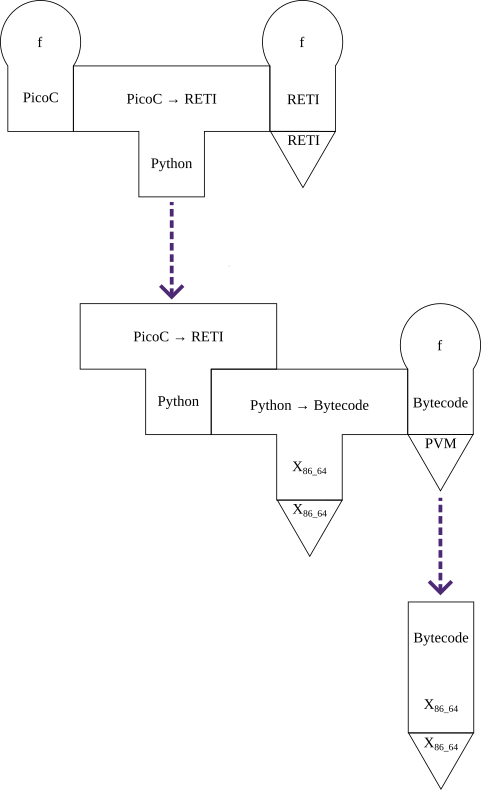
\includegraphics[width=0.5\linewidth]{./figures/summarized_cross_compiler.png}
  \captionof{figure}{Cross-Compiler Kompiliervorgang ausgeschrieben}
}

{
  \centering
  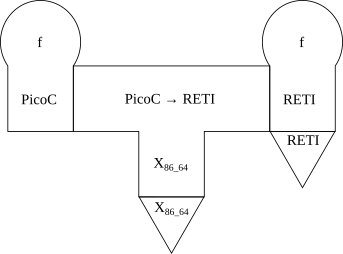
\includegraphics[width=0.33\linewidth]{./figures/compiliervorang_mit_machiene.png}
  \captionof{figure}{Cross-Compiler Kompiliervorgang Kurzform}
}

{
  \centering
  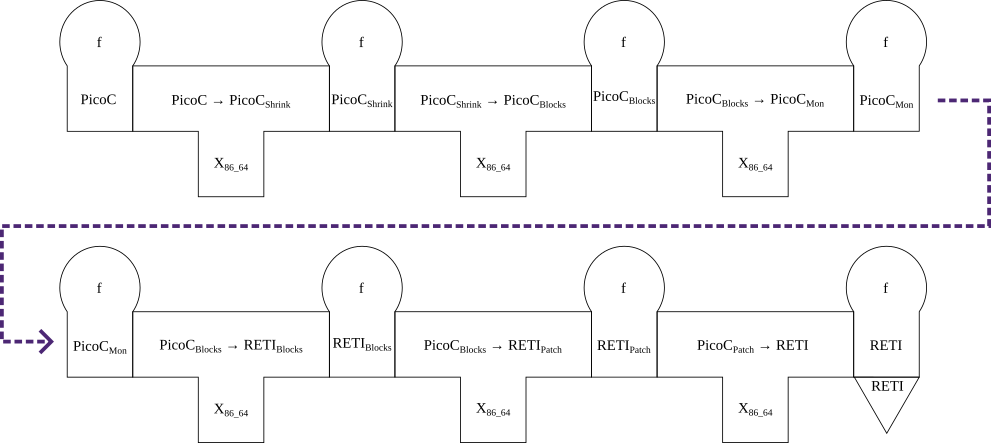
\includegraphics[width=\linewidth]{./figures/passes.png}
  \captionof{figure}{Architektur mit allen Passes ausgeschrieben}
}

\section{Lexikalische Analyse}
\subsection{Verwendung von Lark}
% erwähnen, dass in Lark die Grammatiken L_Lex und L_Parse gemischt sind
% EBNF erwähnen
% (erwähnen, dass finalle Grammatik im Appendix)
\subsection{Basic Parser}
\section{Syntaktische Analyse}
\subsection{Verwendung von Lark}
% Vorteile von Lark
\subsection{Umsetzung von Präzidenz}
Die \colorbold{PicoC Sprache} hat dieselben \colorbold{Präzidenzregeln} implementiert, wie die \colorbold{Sprache C} \footcite{noauthor_c_nodate}. Die \colorbold{Präzidenzregeln} von \colorbold{PicoC} sind in Tabelle~\ref{tab:reference_table} aufgelistet.

\begin{table}[H]
  \center
  \begin{tabulary}{\linewidth}{|C|C|L|L|}
  \toprule
  \colorbold{Präzidenz} &	\colorbold{Operator} & \colorbold{Beschreibung} &	\colorbold{Assoziativität} \\
  \midrule
  1	& \verb|a()|	& Funktionsaufruf & \multirow{2}{=}{Links, dann rechts $\rightarrow$} \\
    & \verb|a[]|	& Indexzugriff & \\
    & \verb|a.b| & Attributzugriff & \\
  \hline
  2	&	\verb|-a| & Unäres Minus & \multirow{2}{=}{Rechts, dann links $\leftarrow$} \\
    & \smalltt{!a $\thicksim$a}	& Logisches NOT und Bitweise NOT & \\
    & \verb|*a &a| & Dereferenz und Referenz, auch Adresse-von & \\
  \hline
  3	& \smalltt{a*b a/b a\%b} &	Multiplikation, Division und Modulo & Links, dann rechts $\rightarrow$ \\
  \cline{1-3}
  4	& \verb|a+b a-b|	& Addition und Subtraktion & \\
  \cline{1-3}
  5	& \verb|a<b a<=b| \verb|a>b a>=b| & Kleiner, Kleiner Gleich, Größer, Größer gleich & \\
  \cline{1-3}
  6 &	\verb|a==b a!=b| & Gleichheit und Ungleichheit & \\
  \cline{1-3}
  7 &	\verb|a&b| & Bitweise UND & \\
  \cline{1-3}
  8 &	\verb|a^b| & Bitweise XOR (exclusive or) & \\
  \cline{1-3}
  9 & \smalltt{a$\mid$b} & Bitweise ODER (inclusive or) & \\
  \cline{1-3}
  10	& \verb|a&&b| &	Logiches UND & \\
  \cline{1-3}
  11	& $a{\mid\mid} b$	& Logisches ODER & \\
  \hline
  12 & \verb|a=b| & Zuweisung & Rechts, dann links $\leftarrow$ \\
  \hline
  13 &	\verb|a,b|& Komma	& Links, dann rechts $\rightarrow$ \\
  \bottomrule
\end{tabulary}
\captionof{figure}{Präzidenzregeln von PicoC}
\label{tab:reference_table}
\end{table}
% erwähnen von Mehrdeutigkeit und Assoziativität
% finalle Grammatik im Appendix
% Crafting Compilers Quelle benennen
\subsection{Derivation Tree Generierung}
\subsection{Early Parser}
\subsection{Derivation Tree Vereinfachung}
% Visitor erwähnen
\subsection{Abstrakt Syntax Tree Generierung}
\subsubsection{ASTNode}
\subsubsection{PicoC Nodes}
% Tabelle aller PicoC Nodes
% möglichst kurze und leicht verständliche Bezeichner für Nodes
\subsubsection{RETI Nodes}
% Tabelle aller RETI Nodes
% Transformer erwähnen
\section{Code Generierung}
\subsection{Passes}
\subsubsection{PicoC-Shrink Pass}
% dieser Pass wurde wegen
\subsubsection{PicoC-Blocks Pass}
\subsubsection{PicoC-Mon Pass}
\begin{Definition}{Symboltabelle}{symboltabelle}
\end{Definition}
\subsubsection{RETI-Blocks Pass}
\subsubsection{RETI-Patch Pass}
\subsubsection{RETI Pass}
% TODO: zusammenfassendes Bild

\subsection{Umsetzung von Pointern}
\subsubsection{Pointer Dereferenzierung durch Zugriff auf Arrayindex ersetzen}
{
  \centering
  \numberedcodebox[minted language=c]{./code_examples/example_pntr_deref.picoc}
  \captionof{figure}{PicoC Code für Pointer Dereferenzierung}
  \label{fig:picoc_code_für_pointer_dereferenzierung}
}

{
  \centering
  \numberedcodebox[minted language=text]{./code_examples/example_pntr_deref.ast}
  \captionof{figure}{Abstract Syntax Tree für Pointer Dereferenzierung}
  \label{fig:abstract_syntax_tree_für_pointer_dereferenzierung}
}

{
  \centering
  \numberedcodebox[minted language=text]{./code_examples/example_pntr_deref.picoc_shrink}
  \captionof{figure}{PicoC Shrink Pass für Pointer Dereferenzierung}
  \label{fig:picoc_shrink_für_pointer_dereferenzierung}
}

\subsubsection{Referenzierung}
% Initialisierung eines Pointers

\subsection{Umsetzung von Arrays}
\subsubsection{Initialisierung von Arrays}
% Stack und Globale Statische Daten
{
  \centering
  \numberedcodebox[minted language=c]{./code_examples/example_array_init.picoc}
  \captionof{figure}{PicoC Code für Array Initialisierung}
  \label{fig:picoc_code_für_array_initialisierung}
}

{
  \centering
  \numberedcodebox[minted language=text]{./code_examples/example_array_init.ast}
  \captionof{figure}{Abstract Syntax Tree für Array Initialisierung}
  \label{fig:abstract_syntax_tree_für_array_initialisierung}
}

{
  \centering
  \numberedcodebox[minted language=text]{./code_examples/example_array_init.picoc_mon}
  \captionof{figure}{PicoC Mon Pass für Array Initialisierung}
  \label{fig:picoc_mon_für_array_initialisierung}
}

{
  \centering
  \numberedcodebox[minted language=text]{./code_examples/example_array_init.reti_blocks}
  \captionof{figure}{RETI Blocks Pass für Array Initialisierung}
  \label{fig:reti_blocks_für_array_initialisierung}
}


% kleines Extra
\subsubsection{Zugriff auf Arrayindex}
Der Zugriff auf einen bestimmten  Index eines Arrays ist wie folgt umgesetzt:

{
  \centering
  \numberedcodebox[minted language=c]{./code_examples/example_array_access.picoc}
  \captionof{figure}{PicoC Code für Zugriff auf Arrayindex}
  \label{fig:picoc_code_für_zugriff_auf_arrayindex}
}

{
  \centering
  \numberedcodebox[minted language=text]{./code_examples/example_array_access.ast}
  \captionof{figure}{Abstract Syntax Tree für Zugriff auf Arrayindex}
  \label{fig:abstract_syntax_tree_für_zugriff_auf_arrayindex}
}

{
  \centering
  \numberedcodebox[minted language=text]{./code_examples/example_array_access.picoc_mon}
  \captionof{figure}{PicoC Mon Pass für Zugriff auf Arrayindex}
  \label{fig:picoc_mon_für_zugriff_auf_arrayindex}
}

{
  \centering
  \numberedcodebox[minted language=text]{./code_examples/example_array_access.reti_blocks}
  \captionof{figure}{RETI Blocks Pass für Zugriff auf Arrayindex}
  \label{fig:reti_blocks_für_zugriff_auf_arrayindex}
}

\subsubsection{Zuweisung an Arrayindex}
{
  \centering
  \numberedcodebox[minted language=c]{./code_examples/example_array_assignment.picoc}
  \captionof{figure}{PicoC Code für Zuweisung an Arrayindex}
  \label{fig:picoc_code_für_array_assignment}
}

{
  \centering
  \numberedcodebox[minted language=text]{./code_examples/example_array_assignment.ast}
  \captionof{figure}{Abstract Syntax Tree für Zuweisung an Arrayindex}
  \label{fig:abstract_syntax_tree_für_array_assignment}
}

{
  \centering
  \numberedcodebox[minted language=text]{./code_examples/example_array_assignment.picoc_mon}
  \captionof{figure}{PicoC Mon Pass für Zuweisung an Arrayindex}
  \label{fig:picoc_mon_für_array_assignment}
}

{
  \centering
  \numberedcodebox[minted language=text]{./code_examples/example_array_assignment.reti_blocks}
  \captionof{figure}{RETI Blocks Pass für Zuweisung an Arrayindex}
  \label{fig:reti_blocks_für_array_assignment}
}

\subsection{Umsetzung von Structs}
\subsubsection{Deklaration von Structs}
{
  \centering
  \numberedcodebox[minted language=c]{./code_examples/example_struct_decl.picoc}
  \captionof{figure}{PicoC Code für Deklaration von Structs}
  \label{fig:picoc_code_für_deklaration_von_structs}
}

{
  \centering
  \numberedcodebox[breakable, minted language=text]{./code_examples/example_struct_decl.st}
  \captionof{figure}{Symboltabelle für Deklaration von Structs}
  \label{fig:symboltabelle_für_deklaration_von_structs}
}

\subsubsection{Initialisierung von Structs}
{
  \centering
  \numberedcodebox[minted language=c]{./code_examples/example_struct_init.picoc}
  \captionof{figure}{PicoC Code für Initialisierung von Structs}
  \label{fig:picoc_code_für_initialisierung_von_structs}
}

{
  \centering
  \numberedcodebox[minted language=text, breakable]{./code_examples/example_struct_init.ast}
  \captionof{figure}{Abstract Syntax Tree für Initialisierung von Structs}
  \label{fig:abstract_syntax_tree_für_initialisierung_von_structs}
}

{
  \centering
  \numberedcodebox[minted language=text]{./code_examples/example_struct_init.picoc_mon}
  \captionof{figure}{PicoC Mon Pass für Initialisierung von Structs}
  \label{fig:picoc_mon_pass_für_initialisierung_von_structs}
}

{
  \centering
  \numberedcodebox[minted language=text]{./code_examples/example_struct_init.reti_blocks}
  \captionof{figure}{RETI Blocks Pass für Initialisierung von Structs}
  \label{fig:reti_blocks_pass_für_initialisierung_von_structs}
}

% Stack und Globale Statische Daten
\subsubsection{Zugriff auf Structattribut}
{
  \centering
  \numberedcodebox[minted language=c]{./code_examples/example_struct_attr_access.picoc}
  \captionof{figure}{PicoC Code für Zugriff auf Structattribut}
  \label{fig:picoc_code_für_zugriff_auf_structattribut}
}

{
  \centering
  \numberedcodebox[minted language=text, breakable]{./code_examples/example_struct_attr_access.ast}
  \captionof{figure}{Abstract Syntax Tree für Zugriff auf Structattribut}
  \label{fig:abstract_syntax_tree_für_zugriff_auf_structattribut}
}

{
  \centering
  \numberedcodebox[minted language=text]{./code_examples/example_struct_attr_access.picoc_mon}
  \captionof{figure}{PicoC Mon Pass für Zugriff auf Structattribut}
  \label{fig:picoc_mon_pass_für_zugriff_auf_structattribut}
}

{
  \centering
  \numberedcodebox[minted language=text]{./code_examples/example_struct_attr_access.reti_blocks}
  \captionof{figure}{RETI Blocks Pass für Zugriff auf Structattribut}
  \label{fig:reti_blocks_pass_für_zugriff_auf_structattribut}
}

\subsubsection{Zuweisung an Structattribut}
{
  \centering
  \numberedcodebox[minted language=c]{./code_examples/example_struct_attr_assignment.picoc}
  \captionof{figure}{PicoC Code für Zuweisung an Structattribut}
  \label{fig:picoc_code_für_zuweisung_an_structattribut}
}

{
  \centering
  \numberedcodebox[minted language=text, breakable]{./code_examples/example_struct_attr_assignment.ast}
  \captionof{figure}{Abstract Syntax Tree für Zuweisung an Structattribut}
  \label{fig:abstract_syntax_tree_für_zuweisung_an_structattribut}
}

{
  \centering
  \numberedcodebox[minted language=text]{./code_examples/example_struct_attr_assignment.picoc_mon}
  \captionof{figure}{PicoC Mon Pass für Zuweisung an Structattribut}
  \label{fig:picoc_mon_pass_für_zuweisung_an_structattribut}
}

{
  \centering
  \numberedcodebox[minted language=text]{./code_examples/example_struct_attr_assignment.reti_blocks}
  \captionof{figure}{RETI Blocks Pass für Zuweisung an Structattribut}
  \label{fig:reti_blocks_pass_für_zuweisung_an_structattribut}
}

\subsection{Umsetzung des Zusammenspiels der Derived Datatypes}
% Allgemeine Form, Start, Mittelteil und Ende
% Umgang mit PntrDecl (inmitten von ArrayDecl)
% Umgang, wenn Datentyp abrubt aufhört am Ende
\subsubsection{Definition von Variablen mit den Derived Datatypes}
% Stack und Globale Statische Daten
{
  \centering
  \numberedcodebox[minted language=c]{./code_examples/example_variable_definition_derived_datatypes_global_static_data.picoc}
  \captionof{figure}{PicoC Code für Definition von Variablen}
  \label{fig:picoc_code_für_definition_von_variablen}
}

{
  \centering
  \numberedcodebox[breakable, minted language=text]{./code_examples/example_variable_definition_derived_datatypes_global_static_data.st}
  \captionof{figure}{Symboltabelle für Definition von Variablen}
  \label{fig:symboltabelle_für_definition_von_variablen}

}

\subsection{Umsetzung von Funktionen}
\subsubsection{Funktionen auflösen zu RETI Code}
\newlineparagraph{Sprung zur Main Funktion}
\subsubsection{Funktionsdeklaration}
\subsubsection{Funktionsdefinition}
\newlineparagraph{Allocation von Variablen}
% Stack und Globale Statische Daten
% die Sache mit Assign(Tmp, Global) und Assign(Global, Tmp)
% erwähnen, das Main Funktion keinen Stackframe hat
% zählen der Größe der lokalen Daten und Parameter
% TODO: Signatur zu Parameter umbenennen
\subsubsection{Funktionsaufruf}
\newlineparagraph{Ohne Rückgabewert}
% Unsichtbares return
{
  \centering
  \numberedcodebox[minted language=c]{./code_examples/example_function_call_no_return_value.picoc}
  \captionof{figure}{PicoC Code für Funktionsaufruf ohne Rückgabewert}
  \label{fig:picoc_code_für_funktionsaufruf_ohne_rückgabewert}
}

{
  \centering
  \numberedcodebox[minted language=text]{./code_examples/example_function_call_no_return_value.picoc_mon}
  \captionof{figure}{PicoC Mon Pass für Funktionsaufruf ohne Rückgabewert}
  \label{fig:picoc_mon_pass_für_funktionsaufruf_ohne_rückgabewert}
}

{
  \centering
  \numberedcodebox[minted language=text]{./code_examples/example_function_call_no_return_value.reti_blocks}
  \captionof{figure}{RETI Blocks Pass für Funktionsaufruf ohne Rückgabewert}
  \label{fig:reti_blocks_pass_für_funktionsaufruf_ohne_rückgabewert}
}

{
  \centering
  \numberedcodebox[minted language=text]{./code_examples/example_function_call_no_return_value.reti}
  \captionof{figure}{RETI Pass für Funktionsaufruf ohne Rückgabewert}
  \label{fig:reti_pass_für_funktionsaufruf_ohne_rückgabewert}
}


\newlineparagraph{Mit Rückgabewert}
{
  \centering
  \numberedcodebox[minted language=c]{./code_examples/example_function_call_with_return_value.picoc}
  \captionof{figure}{PicoC Code für Funktionsaufruf mit Rückgabewert}
  \label{fig:picoc_code_für_funktionsaufruf_mit_rückgabewert}
}

{
  \centering
  \numberedcodebox[minted language=text]{./code_examples/example_function_call_with_return_value.picoc_mon}
  \captionof{figure}{PicoC Mon Pass für Funktionsaufruf mit Rückgabewert}
  \label{fig:picoc_mon_pass_für_funktionsaufruf_mit_rückgabewert}
}

{
  \centering
  \numberedcodebox[minted language=text]{./code_examples/example_function_call_with_return_value.reti_blocks}
  \captionof{figure}{RETI Blocks Pass für Funktionsaufruf mit Rückgabewert}
  \label{fig:reti_blocks_pass_für_funktionsaufruf_mit_rückgabewert}
}

{
  \centering
  \numberedcodebox[minted language=text]{./code_examples/example_function_call_with_return_value.reti}
  \captionof{figure}{RETI Pass für Funktionsaufruf mit Rückgabewert}
  \label{fig:reti_pass_für_funktionsaufruf_mit_rückgabewert}
}

\newlineparagraph{Umsetzung von Call by Sharing für Arrays}

\newlineparagraph{Umsetzung von Call by Value für Structs}
% argmode für Struct Call by Value

\subsection{Umsetzung kleinerer Details}
% langen Sprüngen, großen Konstanten, Division durch 0
\section{Fehlermeldungen}
\subsection{Error Handler}
\subsection{Arten von Fehlermeldungen}
\subsubsection{Syntaxfehler}
\subsubsection{Laufzeitfehler}
% Fehlermeldung ist, wenn der Lexer (partielle Funktion) oder Parser nicht matcht
% Token und Nodes enthalten Position, im Transformer wird die Position von den Token auf die Nodes übertragen und auch die Symboltabelle speichert Position
